\section{Evaluation protocol}
\label{sec:protocol}
Only \texttt{evaluate.py} reads the test split, after every model and rule was fixed; validation sets the temperature,
the threshold, and the ``best mitigation'' (highest validation bias AUC within DistilBERT). Metrics are AUC, toxic-class
F1 and accuracy; the \citet{borkan2019nuanced} bias AUC over subgroup, BPSN and BNSP AUC; the FPR gap between each
identity and the background; worst-group accuracy over 16 identity$\times$label groups \citep{koh2021wilds}; and ECE.
Counterfactual probes use CheckList-style \citep{ribeiro2020beyond} templates (8 neutral, 5 toxic) filled with 18
identity terms, 5 absent from the CDA lexicon, and every in-category swap of 2{,}000 real test comments. TF-IDF and bert-mini numbers carry 95\%
bootstrap intervals over the test set; DistilBERT's three seeds also expose training variance (Table~\ref{tab:seeds}).

\section{Results}
\begin{table*}[t]\centering\small
\resizebox{\linewidth}{!}{\begin{tabular}{lcccccc}\toprule
Model & ROC-AUC $\uparrow$ & F1 $\uparrow$ & Bias AUC $\uparrow$ & Worst-group acc $\uparrow$ & Mean $|$FPR gap$|$ $\downarrow$ & ECE $\downarrow$\\\midrule
B1 majority & 0.500 & 0.000 & 0.500 & 0.000 & 0.000 & 0.114\\
\midrule
B2 ERM & 0.912 {\scriptsize$\pm$0.002} & \textbf{0.599} & \textbf{0.871} {\scriptsize$\pm$0.003} & 0.509 {\scriptsize$\pm$0.022} & 0.103 & 0.015\\
\quad ERM, 80K subsample & 0.894 {\scriptsize$\pm$0.003} & 0.569 & 0.847 {\scriptsize$\pm$0.003} & 0.478 {\scriptsize$\pm$0.023} & 0.124 & 0.024\\
\quad + reweight & 0.884 {\scriptsize$\pm$0.003} & 0.568 & 0.856 {\scriptsize$\pm$0.004} & 0.432 {\scriptsize$\pm$0.023} & \textbf{0.038} & 0.089\\
\quad + CDA & 0.906 {\scriptsize$\pm$0.002} & 0.591 & 0.867 {\scriptsize$\pm$0.003} & 0.509 {\scriptsize$\pm$0.021} & 0.092 & 0.011\\
\quad + soft labels & \textbf{0.914} {\scriptsize$\pm$0.002} & 0.593 & 0.866 {\scriptsize$\pm$0.004} & \textbf{0.604} {\scriptsize$\pm$0.022} & 0.143 & 0.027\\
\quad + combo & 0.889 {\scriptsize$\pm$0.002} & 0.562 & 0.854 {\scriptsize$\pm$0.004} & 0.474 {\scriptsize$\pm$0.023} & 0.070 & \textbf{0.005}\\
\midrule
bert-mini ERM (80K, CPU) & 0.914 {\scriptsize$\pm$0.002} & 0.606 & 0.874 {\scriptsize$\pm$0.003} & 0.510 {\scriptsize$\pm$0.035} & 0.077 & \textbf{0.007}\\
\quad + reweight & 0.896 {\scriptsize$\pm$0.002} & 0.567 & 0.866 {\scriptsize$\pm$0.003} & 0.419 {\scriptsize$\pm$0.048} & \textbf{0.028} & 0.158\\
\quad + CDA & 0.914 {\scriptsize$\pm$0.002} & 0.605 & 0.874 {\scriptsize$\pm$0.003} & 0.546 {\scriptsize$\pm$0.029} & 0.094 & 0.012\\
\quad + group DRO & 0.862 {\scriptsize$\pm$0.002} & 0.487 & 0.834 {\scriptsize$\pm$0.004} & 0.171 {\scriptsize$\pm$0.018} & 0.048 & 0.276\\
\quad + soft labels & \textbf{0.920} {\scriptsize$\pm$0.002} & \textbf{0.613} & 0.880 {\scriptsize$\pm$0.003} & \textbf{0.567} {\scriptsize$\pm$0.024} & 0.084 & 0.013\\
\quad + combo & 0.914 {\scriptsize$\pm$0.002} & 0.598 & \textbf{0.882} {\scriptsize$\pm$0.003} & 0.563 {\scriptsize$\pm$0.025} & 0.050 & 0.044\\
\midrule
B3 DistilBERT ERM & 0.940 {\scriptsize$\pm$0.002} & 0.659 & 0.905 {\scriptsize$\pm$0.003} & 0.614 {\scriptsize$\pm$0.039} & 0.085 & \textbf{0.007}\\
\quad + reweight & 0.930 {\scriptsize$\pm$0.002} & 0.635 & 0.902 {\scriptsize$\pm$0.003} & 0.496 {\scriptsize$\pm$0.037} & \textbf{0.025} & 0.110\\
\quad + CDA & 0.939 {\scriptsize$\pm$0.002} & 0.656 & 0.904 {\scriptsize$\pm$0.003} & 0.606 {\scriptsize$\pm$0.029} & 0.075 & 0.011\\
\quad + group DRO & 0.914 {\scriptsize$\pm$0.002} & 0.581 & 0.886 {\scriptsize$\pm$0.003} & 0.345 {\scriptsize$\pm$0.026} & 0.026 & 0.191\\
\quad + soft labels & \textbf{0.943} {\scriptsize$\pm$0.002} & \textbf{0.661} & \textbf{0.910} {\scriptsize$\pm$0.003} & \textbf{0.641} {\scriptsize$\pm$0.027} & 0.084 & 0.009\\
\quad + combo & 0.937 {\scriptsize$\pm$0.002} & 0.640 & 0.908 {\scriptsize$\pm$0.003} & 0.596 {\scriptsize$\pm$0.029} & 0.039 & 0.039\\
\bottomrule\end{tabular}}
\caption{Test results (WILDS test, 132,607 comments). Thresholds and temperatures are fit on validation; $\pm$ is half the 95\% bootstrap interval (50 resamples of the test set; it does not include training-seed variance). Bias AUC is the \citet{borkan2019nuanced} final metric (generalised mean, $p{=}{-}5$, of subgroup, BPSN and BNSP AUC, averaged with overall AUC). Worst-group accuracy is the minimum over the 16 identity$\times$label groups. FPR gap is identity-group FPR minus background FPR. Bold marks the best value within each model family.}\label{tab:main}
\end{table*}
Tables report seed 0; claims about differences between DistilBERT mitigations use the three-seed means in
Table~\ref{tab:seeds}. The counterfactual, per-identity and calibration results are in Appendix~\ref{app:more}.

\paragraph{Model family matters more than any mitigation.} DistilBERT on the full split beats both cheaper families on
AUC, F1, bias AUC and worst-group accuracy (Table~\ref{tab:main}): AUC \BertDistilErmAuc{} vs.\ \TfidfErmAuc{}
(TF-IDF) and \BertErmAuc{} (bert-mini), and bias AUC \BertDistilErmBiasAuc{} vs.\ 0.871 and 0.874. Data size explains
part of this: TF-IDF trained on the 80K subsample drops to AUC 0.894. The likely main reason is pretraining: both
transformers start from language models that already encode English syntax and semantics, so fine-tuning only has to
map that knowledge onto toxicity, while TF-IDF must learn every word association from the labelled comments alone.
Consistent with this, bert-mini on 80K comments beats TF-IDF on the same 80K (\BertErmAuc{} vs.\ 0.894) and matches
TF-IDF trained on all \NTrain{}.

\paragraph{Soft labels are the only mitigation that never lowers AUC.} In all three families, soft labels give the
highest AUC and the best worst-group accuracy, with accuracy within 0.01 of ERM. Bias AUC improves for both
transformers (bert-mini 0.874 $\rightarrow$ 0.880; DistilBERT 0.905 $\rightarrow$ 0.909, seed s.d.\ 0.0004) but not
for TF-IDF (0.871 $\rightarrow$ 0.866). DistilBERT's worst-group accuracy rises from 0.58 to 0.62, within its seed
s.d.\ of 0.03. The validation rule picks \Best{} as the best mitigation. Soft labels do \emph{not} shrink the FPR gap
(\BertDistilSoftMeanAbsFprGap{} vs.\ \BertDistilErmMeanAbsFprGap{}): identity comments are ranked better but flagged
as often.

\paragraph{Reweighting and group DRO buy small FPR gaps with missed toxicity.} Both shrink DistilBERT's mean FPR gap
about threefold (0.075 $\rightarrow$ 0.023 and 0.029; DRO even flags identity comments \emph{less} often than background
ones), but both lose AUC and bias AUC in every family they run in (Figure~\ref{fig:tradeoff}). Worst-group accuracy
falls to 0.48 and 0.35 because toxic comments about each group are missed more often (Table~\ref{tab:identity}), and
calibration breaks beyond what temperature scaling repairs (ECE 0.110 and 0.191 vs.\ 0.007 for ERM), because
reweighting changes the effective base rate.

\paragraph{CDA fixes the words it saw.} Augmentation cuts the score change under identity swaps of real comments two-
to fourfold in every family (DistilBERT \BertDistilErmCfRealDelta{} $\rightarrow$ 0.012; Table~\ref{tab:cf}) but leaves
the test metrics and the FPR gap essentially unchanged, and it does not transfer to held-out identity terms
(DistilBERT template spread 0.088 without CDA, 0.094 with). The real-comment probe uses the augmentation's own
lexicon, so the held-out templates are the fairer test.

\paragraph{Combining.} The pre-registered combo halves the FPR gap (0.034) with bias AUC 0.909, AUC within 0.003 of
ERM and the lowest swap sensitivity (0.009), but worse worst-group accuracy (0.56) and calibration (ECE 0.039) than soft
labels alone: the better trade if avoiding silenced identity speech matters most.

\begin{table}[t]\centering\small\setlength\tabcolsep{2.5pt}
\resizebox{\linewidth}{!}{\begin{tabular}{lccccc}\toprule
DistilBERT & AUC & F1 & Bias AUC & Worst-gr. & $|$FPR gap$|$\\\midrule
erm (3) & 0.940{\scriptsize$\pm$0.000} & 0.658{\scriptsize$\pm$0.000} & 0.905{\scriptsize$\pm$0.000} & 0.584{\scriptsize$\pm$0.030} & 0.075{\scriptsize$\pm$0.012}\\
cda (3) & 0.939{\scriptsize$\pm$0.000} & 0.656{\scriptsize$\pm$0.001} & 0.905{\scriptsize$\pm$0.000} & 0.598{\scriptsize$\pm$0.014} & 0.072{\scriptsize$\pm$0.008}\\
reweight (3) & 0.930{\scriptsize$\pm$0.001} & 0.632{\scriptsize$\pm$0.003} & 0.902{\scriptsize$\pm$0.001} & 0.477{\scriptsize$\pm$0.016} & 0.023{\scriptsize$\pm$0.004}\\
dro (3) & 0.914{\scriptsize$\pm$0.000} & 0.577{\scriptsize$\pm$0.003} & 0.887{\scriptsize$\pm$0.001} & 0.353{\scriptsize$\pm$0.024} & 0.029{\scriptsize$\pm$0.002}\\
soft (3) & 0.943{\scriptsize$\pm$0.000} & 0.663{\scriptsize$\pm$0.002} & 0.909{\scriptsize$\pm$0.000} & 0.621{\scriptsize$\pm$0.032} & 0.078{\scriptsize$\pm$0.008}\\
combo (3) & 0.937{\scriptsize$\pm$0.000} & 0.645{\scriptsize$\pm$0.004} & 0.909{\scriptsize$\pm$0.000} & 0.558{\scriptsize$\pm$0.034} & 0.034{\scriptsize$\pm$0.007}\\
\bottomrule\end{tabular}}
\caption{DistilBERT across training seeds: mean $\pm$ standard deviation (number of seeds in parentheses). Each seed gets its own validation temperature and threshold.}\label{tab:seeds}
\end{table}
\begin{figure}[t]\centering
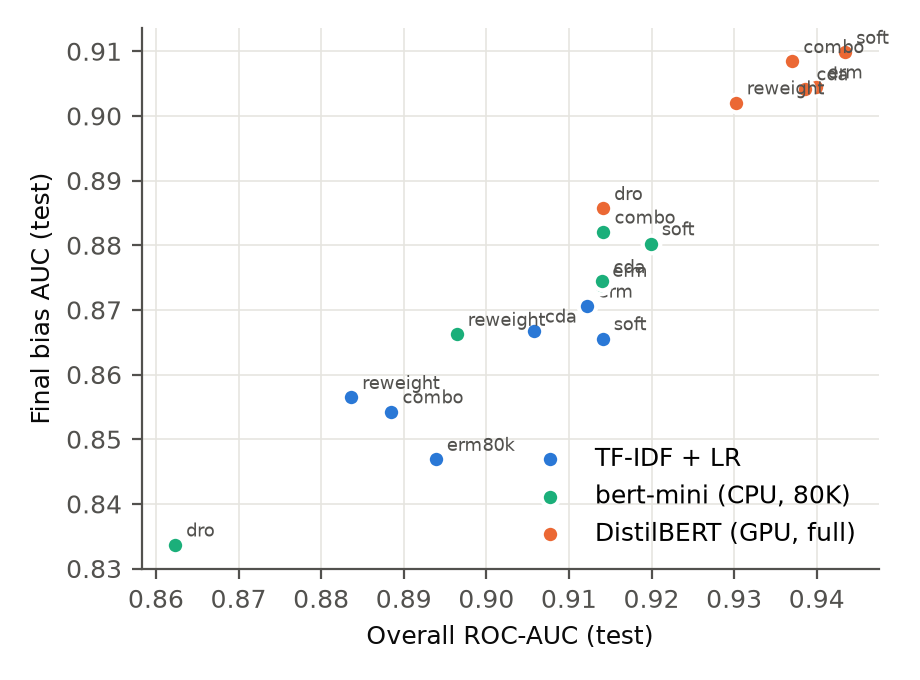
\includegraphics[width=\columnwidth]{../results/fig_tradeoff.png}
\caption{Overall AUC against bias AUC on test for every model (seed 0). Within each family, reweighting and DRO move
down and to the left; soft labels move right, and also up for the two transformers.}\label{fig:tradeoff}
\end{figure}

\paragraph{Templates and deferral.} DistilBERT ERM flags 19\% of the 144 neutral identity sentences (``I'm proud to be
gay.''); reweighting and DRO bring this to 3.5\% and 0\%, and every DistilBERT model except DRO flags all 90 toxic
ones. TF-IDF's neutral sentences about \emph{gay} average $P(\text{toxic}){=}0.70$ (Figure~\ref{fig:templates}).
After temperature scaling, ERM and soft-label DistilBERT are well calibrated (ECE \BertDistilErmEceCal{} and
\BertDistilSoftEceCal{}), and deciding only the 80\% of comments furthest from the threshold cuts the error rate from
0.083 to \BertDistilErmErrAtEightycov{} and \BertDistilSoftErrAtEightycov{} (Figure~\ref{fig:rc}). That is what makes
the defer band useful rather than cosmetic.

\section{Error analysis}
\label{sec:errors}
\paragraph{Errors live where raters disagree.} Heuristic tags on every test comment (Table~\ref{tab:tags}) show that
92\% of DistilBERT's false negatives and 56\% of its false positives have a borderline label (30--70\% of raters said
toxic), against 13.5\% of correct predictions, and identity mentions appear in 61\% of errors against 37\% of correct
predictions.

\begin{table}[t]\centering\small
\resizebox{\linewidth}{!}{\begin{tabular}{lrrr}\toprule
Reason (hand-coded) & FP & FN & Total\\\midrule
Harsh but civil disagreement & 27 & 24 & 51\\
Implicit or coded hostility & 0 & 30 & 30\\
Identity mention, not hostile & 28 & 0 & 28\\
Gold label looks wrong & 11 & 12 & 23\\
Sarcasm or irony & 7 & 13 & 20\\
Genuinely ambiguous & 12 & 6 & 18\\
Quoting or reporting toxicity & 8 & 9 & 17\\
Rude words, not aimed at anyone & 7 & 1 & 8\\
Other: disguised insult or truncation & 0 & 5 & 5\\
Total & 100 & 100 & 200\\
\bottomrule\end{tabular}}
\caption{Main reason for each of 200 test errors of the best model (100 false positives and 100 false negatives, sampled at random), labelled by hand by the author. One label per error.}\label{tab:hand}
\end{table}
\paragraph{Hand coding: why the errors happen.} To check the tags, I took a random sample of 100 false positives and
100 false negatives of the best model and labelled each by hand with the single reason that best explains it, using
categories fixed before coding (Table~\ref{tab:hand}; each count is also a percentage, with a 95\% interval of at most
$\pm$10 points). The two error types have different causes. The largest false-positive group is non-hostile identity
mentions (\HandFPIdentity{}), the failure the mitigations target, and no false negative falls in it. The largest
false-negative group is implicit or coded hostility (\HandFNImplicit{}): stereotypes and dehumanising remarks without
insult words, followed by sarcasm (\HandFNSarcasm{}). Harsh but civil disagreement accounts for \HandFPCivil{} false
positives and \HandFNCivil{} false negatives, so the model and the raters draw the line between criticism and
incivility in different places, in both directions. I judged the gold label wrong in \HandGoldWrong{} errors and could
not decide in \HandAmbiguous{} more; the mislabelled false positives include a slur that 44\% of its 70 raters called
toxic and a comment implying gay men are predators that none of its four raters did. The last \HandOther{} false
negatives are insults the model cannot read: disguised or abbreviated profanity (``fcking'', ``\#\$\%\#ing'',
``POS''), a misspelling (``maroon''), and a slur past the 128-wordpiece cut.

The heuristic tags overstate identity and miss sarcasm. The identity tag fires on \HandIdTagFP{} sampled false
positives, but by hand the identity mention was the cause in only \HandFPIdentity{}; the quote tag catches
\HandQuoteTag{} quoting errors but also fires on \HandQuoteTagElse{} others; and the sarcasm tag catches only
\HandSarcTag{} sarcastic errors.

\paragraph{Confident false positives and attribution.} The most confident identity ``false positives'' are often
label noise: ``You are a NASTY WOMAN'' was called toxic by 32\% of 65 raters. For ERM the top integrated-gradients
word in these comments is usually an insult; an identity term is the top word in only \IGTopErm{} of the 150 most
confident identity-mentioning false positives (top three: \IGTopThreeErm{}). For the soft-label model these rise to
\IGTopBest{} and \IGTopThreeBest{}. A plausible explanation is that soft targets reproduce the raters' own partial
sensitivity to identity mentions: \BenignIdRater{} of benign training comments that mention an identity have at least
one rater calling them toxic, against \BenignNoIdRater{} of those that mention none (mean toxicity fraction
\BenignIdFrac{} vs.\ \BenignNoIdFrac{}). A thresholded label discards that signal; a soft label keeps it. Testing the
explanation directly needs per-rater labels.

\begin{table}[t]\centering\small\setlength\tabcolsep{3pt}
\resizebox{\linewidth}{!}{\begin{tabular}{lrrrrrr}\toprule
& \multicolumn{3}{c}{False positives} & \multicolumn{3}{c}{False negatives}\\
DistilBERT & fixed & new & total & fixed & new & total\\\midrule
ERM & & & 6,666 & & & 4,399\\
+ CDA & 1,647 & 1,226 & 6,245 & 509 & 779 & 4,669\\
+ reweight & 1,960 & 1,781 & 6,487 & 562 & 1,197 & 5,034\\
+ group DRO & 2,945 & 3,660 & 7,381 & 808 & 2,291 & 5,882\\
+ soft labels & 945 & 1,494 & 7,215 & 687 & 369 & 4,081\\
+ combo & 1,586 & 2,682 & 7,762 & 894 & 823 & 4,328\\
\bottomrule\end{tabular}}
\caption{Test errors of each DistilBERT mitigation against ERM (seed 0, each model at its own validation threshold). \emph{fixed}: ERM errors the mitigation gets right; \emph{new}: errors ERM did not make.}\label{tab:fixed}
\end{table}
\paragraph{Every mitigation trades errors.} Against ERM, soft labels fix \FPFixed{} false positives and \FNFixed{}
false negatives but introduce \FPIntro{} and \FNIntro{} new ones (Table~\ref{tab:fixed}). Every mitigation changes
thousands of individual decisions, even where the totals barely move. Reweighting and group DRO introduce the most new
false negatives, and DRO ends with more false positives than ERM overall: it closes the gap without reducing false
alarms. Soft labels and combo are the only mitigations that miss fewer toxic comments than ERM.

\section{The Fair-Mod workbench}
\label{sec:system}
The Gradio app \citep{abid2019gradio} has three tabs. \emph{Moderate} takes typed text or a comment from a queue that
mixes curated hard cases with real test comments chosen by rule (benign identity mentions ERM flags, likely label
noise, missed toxic comments, 50/50 rater splits). For the selected model it shows the calibrated probability against
the model's threshold, a flag/allow/defer decision from a moderator-set band, subtype probabilities, word
attributions, an identity-swap table with the decision for each swap, and, for queue comments, how the raters split.
Further tabs show per-identity test results and the tool's limitations. Everything is computed live.

\section{Discussion}
\paragraph{What the results support.} (1) A stronger pretrained encoder trained on more data reduces identity-related
ranking errors more than any mitigation applied to a weaker model. (2) Soft labels improve ranking quality without lowering
AUC anywhere: higher AUC and worst-group accuracy in all three families, and higher bias AUC for both transformers,
stable across DistilBERT seeds. (3) The FPR gap can be closed, but only by mitigations that raise false negatives on
the same groups and degrade calibration; which of the two errors matters more is a policy choice, not a modelling
result. (4) CDA makes models invariant to the swaps they were trained on and little else.

\paragraph{What they do not support, and limitations.} The audit covers \emph{mentions} of eight coarse groups, not
authors, and says nothing about dialect-based bias \citep{sap2019risk}. Bias AUC differences between DistilBERT
mitigations are small (0.887--0.909) even where they exceed seed noise. The 19\% template flag rate comes from 144
hand-written sentences, so it shows a problem rather than a deployment rate. ``Correct'' means agreeing with a
majority of usually four raters. The swap lexicon also fires on non-identity uses (``black hole'' becomes ``white hole''); the hand coding
has a single coder (the author), so there is no inter-annotator agreement; bert-mini rests on one seed; and
calibration is fit on the same distribution it is tested on.

\paragraph{Next steps.} (1) Test the soft-label hypothesis with per-rater labels, for example by holding out the rater
votes of identity-mentioning comments. (2) Guide CDA with named entity recognition, which tags mentions of nationalities
and religious or political groups, so that only terms referring to people are swapped (no ``white hole''), and add
held-out identities to training. (3) Make the threshold group-aware or add a reject-option rule, which could close the FPR gap without
retraining. (4) Normalise disguised profanity and score long comments in windows, since both explain missed toxic
comments in the hand-coded sample. (5) Evaluate transfer to a second dataset.

\section{Ethics}
The data is public, CC0, and released without user ids; quotes are short and not traceable to authors, and the app
and paper carry content warnings. ``Toxicity'' encodes a particular rater pool's norms, which the model inherits. The
tool is decision support with a defer option, because a ``debiased'' classifier could give automated removal false
legitimacy.

\section{Generative AI disclosure}
I used Claude Opus 5.5 to generate initial implementations for multiple scripts throughout my pipeline and to toubleshoot errors in them as well as hunt for bugs and fix them. I made sure that I understood every line of generated code and have heavily revised the code manually to match my dataset. I frequently tested generated code manually to ensure that it worked as intended and never blindly trusted generated code. Claude was also used to design my slides. However, all content within the slides was generated by me manually and I told Claude exactly what to put on each slide and with what format. Claude also generated all Latex code I used. I know how to use latex myself and I was the one that instructed claude to build the pdf using latex. However, I am not fast at writing latex so I instead wrote the entirety of the report on a google doc which I then gave to claude for the purposes of transforming it into latex code. When it comes to prose, claude was used for syntactical, vocabulary, grammar, and spelling corrections, after my report was already complete. The part of my report referencing Named Entity Recognition models was suggested to me by my TA as feedback during the oral defense. 

\section*{Reproducibility}
{\raggedright Code: \url{https://github.com/taxpet06/fair-mod}; data: the CC0 WILDS mirror in Section~\ref{sec:data}.
The README gives setup, pinned requirements, and run times. After \texttt{pip install -r requirements.txt} and
\texttt{./download\_data.sh}, the analysis runs as \texttt{tfidf.py}, \texttt{bert.py} per variant, \texttt{evaluate.py},
\texttt{errors.py}, and \texttt{report/build\_tables.py}; \texttt{app.py} starts the workbench. Seeds are fixed.
Tables and macro numbers are generated from \texttt{results/}; other numbers were typed from the same CSVs, except the
proposal's exploration figures and the laptop throughputs.\par}
